\section{Verification}
The exact meaning of verification is confusing \cite{thomas_arts}. The
definition may differ in comparison of academic or industrial use. Even in
different phases of the safety life cycle verification is conducted in various
forms \cite[8:9.2]{ISO26262}.

\subsection{Formal Verification}
%Skriv n�got luddigt
\subsection{Semi formal verification}
%Skriv n�got �n mer luddigt

\section{Industrial Safety Standards} It is useful to distinguish between
systems with different levels of dependability, and determine where the hazards
exists\cite{COURSEBOOK:safety-critical}. When this risk analysis is completed
%% �verv�g kommatecken mellan dessa satser
and appropriate reliability and availability requirements is assigned to the
system, the system can be identified by a certain safety integrity level (SIL).
If this number is high, the system will experience a more rigorous design and
testing than could be justified for a lesser demanding system. These levels is
more defined in standards IEC~61508 and ISO~26262.

%\setion{Functional Safety}
% Kanske n�got vi vill skriva om? N�ms i metoden

\subsection {IEC~61508 and ISO~26262}

%G�r skillnad p� verifikation och verifikation. Dvs vilken fas handlar det om?
Automotive software for safety related systems is required to be designed,
implemented and verified by the standard ISO~26262, which handles functional
safety for automotive equipment. For a higher level of integrity ISO~26262
strongly recommends that semi formal verification of each module should be
executed \cite[Part 6]{ISO26262}.  It also recommends a formal verification, but
because of the state-space complexity this is hard to achieve.

ISO~26262 is built on IEC~61508 which is titled Functional Safety of
Electrical/Electronic/Programmable Electronic Safety-related Systems. IEC~61508
can be applied to any kind of industry while ISO~26262 is defined only for the
automotive industry. IEC~61508 have four safety integrity levels (SIL) ranked
1-4. SIL 4 is the highest and should be applied where a failure can
do devastating damage to a large area. %% �r det inte ocks� s� att om det �r
%% ganska farligt men riskerar att h�nda ofta s� ska den ocks� klassas som SIL 4.
The automotive industry is improbable to have this risk. That is why ISO~26262
%% "that is why" - syftar p� att detta �r huvudanledningen. det �r nog m�nga
%% olika anledningar att ISO26262 har utvecklats.
exists which also defines four levels of SIL called automotive safety integrity
level (ASIL). The ASIL range from A-D, where D is the highest and roughly
translate to SIL 3.

\subsection{AUTOSAR (AUTomotive Open System ARchitecture)}
%Beskriv vad fan det �r
%K�lla http://www.autosar.org/
AUTOSAR is a worldwide development partnership of car manufacturers, suppliers
and other companies from the electronics, semiconductor and software industry.

Some of the specifications in AUTOSAR is left quite open for interpretation.
%% beskriv varf�r dessa inte �r tillr�ckligt definierade, och varf�r olika
%% konfigurationer existerar.
This makes it possible for vehicle developers to have different specifications
for a configuration. Some parts of those configuration specifications is
generated into code, while other is manually written or added as a configurable.

\section{Existing Software}
There are a number of existing software tools whose aim are to simplify the
implementation of verification and testing.
%% ..och helt pl�tsligt presenteras en lista av n�got..
\begin{itemize}
\item QuickCheck
\item SPIN
\item McErlang
\item $\mu$CRL toolset
\item CADP
\item Parasoft C/C++test
%\item Erlang and QuickCheck
%\item Symlink
%\item CORE
%\item Isabelle
\end{itemize}

\subsection{QuickCheck}
Quickcheck was invented be Koen Claessen and John Hughes, as a testing module
for Haskell, in 2000.
In 2006 John Hughes founded the Company Quviq together with
Thomas Arts. Quviq offers a commercial version of Quickcheck for Erlang.
The main difference, except from the programming paradigms, is that
the commercial version of Quickcheck has a C-testing interface. Hence it
possible to test C-code in Erlang with help of QuickCheck. All code for tests
is written in Erlang and checked against API calls to the C-code. It is actually
not necessary to have actual source code; it is enough to only have compiled library
files.

QuickCheck tests a program with specification implemented as properties that
the program must hold \cite{QUICKCHECK:manual}. QuickCheck has guided random
test generation, this means that the samples can be weighted to cover certain
parts of the state-space with more likelihood.

\lstset{language=erlang}

\subsubsection{Introductions to QuickCheck}
When testing C code with QuickCheck one uses state based testing. Which means
that a model state $S$ is passed around and checked against API calls according to
figure \ref{FIG:API_CALLS}.

\begin{figure}[!h]
\label{FIG:API_CALLS}
\caption{Shows state based testing against API and model state}
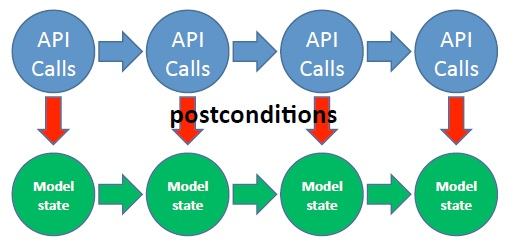
\includegraphics{pictures/api_calls.jpg}
\end{figure}

A property in quickcheck is written in the following way.
\lstset{language=erlang}
\begin{lstlisting}
prop() ->
  ?FORALL(Cmds,commands(),
          begin
            ... = run_commands(Cmds)
          end).

command(S) ->
      [{call, Mod, CFunction, arg_generator(S)},
        ... ].
\end{lstlisting}

Every commands has, additional to the command definition,
a precondition, postcondition and a next state function, see
paragraph \ref{PAR:EQC_STATEM}.

A property is then tested as:

\begin{lstlisting}
eqc:quickcheck(eqc:numtest(N,prop())).
\end{lstlisting}

Alternative the model states can be shown.

\begin{lstlisting}
eqc:quickcheck(eqc:numtest(N,eqc_statem:show_states(prop()))).
\end{lstlisting}

\subsubsection{Quickcheck Modules}
The commercial version Quickcheck consist of several Erlang modules.
%%eqc
\paragraph{eqc}
The module \emph{eqc} is the main Quickcheck module. This module defines a lot
of macros that can be used when writing properties and also the basic function
like \emph{quickcheck}.
\begin{lstlisting}
    Some Erlang code
\end{lstlisting}

\paragraph{eqc\_gen} Used for generation of test cases.
\begin{lstlisting}
    Some Erlang code
\end{lstlisting}

%%% eqc_c
\paragraph{eqc\_c} Contains the C-testing interface. In other words how to
communicate with C-code.

\begin{lstlisting}
  eqc_c:start(suit,[{c_src,"suit_api.h"},{additional_files,["myprog.o"]}])
\end{lstlisting}
The code above starts the C-program \emph{myprog.o} and a Erlang module
\emph{suit}, the name of the first parameter, is created. This module can now be
used within Erlang to get information about the C-program. For example the
following function, that counts the number of spaces in a string, might be
declared in \emph{suit\_api.h} and defined in the \emph{myprog.o}.
\lstset{language=C}
\begin{lstlisting}
extern int spaces(char *str)
\end{lstlisting}
Then we can make the following call in the Erlang:
\lstset{language=Erlang}
\begin{lstlisting}
suit:spaces("this is a string")
\end{lstlisting}
If the function \emph{spaces} is defined correctly the output will be 3.
%%% eqc_statem
\paragraph{eqc\_statem}
\label{PAR:EQC_STATEM}
Offers state based testing. A command has a definition, precondition,
postcondition, and a next function. If we wanted to test \emph{spaces} function
one may have written.
\begin{lstlisting}

% Defines the initial model state
initial_state() ->
  [].

% Takes the model state as a parameter
% Returns a tuple of the format
%   {call,Module,Function_to_call,Arguments_to_function}
spaces_command(_State) ->
  % Generates a natural number, binds it to Pat and generates a
  % list with length Pat with elements of type char
  Xs = ?LET(Pat,nat(),vector(Pat,char())),
  {call,?MODULE,spaces,[Xs]}.

% The actual call to the C-code
spaces(Xs) ->
  suite:spaces(eqc_c:create_string(Xs)).

%Takes the model state as a parameter
%The spaces function has no pre conditions
spaces_pre(_State) ->
  true.

%Pramaters: S = ModelState, Args = arguments to the command
%Defines what should hold after the command
spaces_post(_S,Args=[Arg],Ret) ->
  length(lists:filter(fun(X) -> X == 32 end,Arg)) == Ret.

%Parameters: S    = model sate before the call,
%            Ret  = return value from command,
%            Args = argements to command
%Return the new model sate after the command is called
spaces_next(S,_Ret,_Args) ->
  S.
\end{lstlisting}

Noticeable is that only the post function may depend on the C-code. QuickCheck
has a generation step where tests are generated according to the precondition
and the model state. The C-code is run first after the generation step and can
only be used to check post conditions. This is actually what one want because it
seems pointless to test a program according to how the same program is executed.

The example above is actually not state dependent since \emph{spaces} only
depend on the argument string. However one can imagine the same function being
dependent on some global variable and according to that variable change its output.
%car_xml
\paragraph{car\_xml}
Additional to the commercial version is \emph{car} module. This module is
specifically created to parse AUTOSAR XML configuration files.
\begin{lstlisting}
    Some Erlang code
\end{lstlisting}

\paragraph{Other modules}
There are also other modules; for instance a module for mocking C-code. Or in
other words, if one has a C-function that is declared but the
definition is missing, one can simulate its output. This is
however not used in this thesis.

%% Erlang �r inget verktyg per se. vi borde skriva om det, men passar det in
%% h�r?
\subsection{Erlang}
Erlang can easily communicate with other programming language by
using byte streams. There have been some work done including Erlang,
AUTOSAR and QuickCheck, mostly by the QuviQ company\cite{QUVIQ:flyer}.
%% "mostly"? skriva n�got om Volvo och SP ocks�?
Imperative coding requires state based testing(?). QuviQ have developed a library in
Erlang for this purpose(?).

% \subsection{CORE}
% A specification package developed by British Aerospace and System Designers.

%\subsection{Promela}

\subsection{SPIN}
SPIN is used to trace logical design errors in distributed
software\cite{SPIN:manual}. It supports a high level language, Promela, to
specify system descriptions. Promela is an acronym for PROcess MEta LAnguage, and
is a verification model language. The system properties that should be checked
are written in logical temporal language (LTL), and SPIN reports errors such as
deadlocks, race conditions and incompleteness between these properties and the
system model. It also supports embedded C code as part of the model
specifications. It supports random, interactive and guided simulation, with both
partial and exhaustive proof techniques.

\subsection{McErlang}
McErlang is a model checker written in Erlang used for verifying distributed
Erlang programs\cite{MCERLANG:model-checker}. Its purpose is to check a program
against a correctness property, but can also among other things check safety
or liveness properties.

McErlang offers two depth-first state traversal model checking algorithms; one
checks safety properties and the other is used for checking the liveness
properties. McErlang also implements weak process fairness, by omitting non-fair
loops from the accepting runs in its liveness algorithm.

%% jag tror mcerlang ing�r i quickcheck suiten. den blir installerad tillsammans
%% med quickcheck iaf.

\subsection{$\mu$CRL toolset} $\mu$CRL is a process algebraic language which is
suited for the analysis of distributed systems. The toolkit is built on this
language and contains a theorem prover based on binary decision
diagrams\cite{MCRL:manual}.

\subsection{CADP} Construction and Analysis of Distributed Processes (CADP),
formerly CAESAR/ALDEBARAN Development Package, is a toolset for the design of
distributed systems\cite{CADP:manual}. It includes, among others, tools for
equivalence checking, state-space manipulation and model checking, and it also
includes several verification algorithms. It provides functionality as
step-by-step simulation to parallel model checking.

\subsection{Parasoft C++test}
Parasoft C++ is a commercial software with a huge range of functionality,
developed by the Parasoft company, with the purpose of testing software written
in C or C++. Parasoft claims that it should be possible to satisfy ASIL
requirements using their software(?).
%\subsection{Isabelle}
% Isabelle theorem prover is an interactive theorem prover, successor of the
% Higher Order Logic (HOL) theorem prover

\section{Verification Methods}
The standard IEC~61508 propose two methods to say that a program is formal
verified. The key is to model the program into one of the following machines.

\begin{enumerate}
\item \label{enum:FSM} Finite state machines/state transition diagrams
\item Time Petri nets
\end{enumerate}

IEC~61508 emphasises that Time Petri nets are best suited for concurrent
programs. Regarding method \ref{enum:FSM} the following criteria needs to be
satisfied for the implemented state machine to be formal verified:

\begin{description}
\item[completeness] the system must have an action and new state for every input
in every state,
\item[consistency] only one state change is described for each state/input
pair, and
\item[reachability] whether or not it is possible to get from one state to
another by any sequence of inputs.
\end{description}

If the state machine is correctly implemented it exist a correct model of the
%% det �r n�got konstigt med denna meningen men jag kan inte riktigt s�tta
%% fingret p� det.
%% kan vara att: om SM �r korrekt implementerad - s� �r originalprogrammet
%% formellt verifierat. �r detta verkligen allt som kr�vs?
original program, then the original program is formal verified.

Since most program specification are written in natural languages there may be
lots of ambiguities. Consequently a lot of techniques has been developed to reduce
such cases. These techniques are often referred to as semi formal verification,
because they lack of mathematical rigour associated with formal
verification. These methods use textual, graphical or other notation; often
several techniques are used in unity. % These tests may not be

The description of semi formal verification in IEC~61508 states: \\
''Semi-formal methods provide a means of developing a description of a system at
some stage in its development, i.e. specification, design or coding. The
description can in some cases be analysed by machine or animated to display
various aspects of the system behaviour.''
